%% =====================================================================
%%  MLEE Course Project Poster Template  (BITS Pilani, EEE Department)
%%  Format : A0 portrait, tikzposter class
%%  Build  : pdflatex MLEE_Poster_Template.tex   (run twice)
%%
%%  HOW TO USE
%%  1. Put the BITS logo in this folder as  bits_logo.png  (or .pdf/.jpg
%%     and edit \biTSlogofile below). The dashed placeholder is replaced
%%     automatically once the file exists.
%%  2. Edit title, authors, instructor, team ID in the preamble.
%%  3. Replace the guideline text in every block with your own content.
%%  4. Replace each figure placeholder: save your plots as fig_method.png,
%%     fig_result1.png, fig_result2.png (or change the names in \figslot).
%%  5. Delete the "Poster Guidelines" block before printing.
%%
%%  The poster and the written report are complementary and equally
%%  weighted. Keep title, numbers, terminology and key figures identical.
%% =====================================================================
\documentclass[30pt, a0paper, portrait, margin=0mm, innermargin=15mm,
               blockverticalspace=15mm, colspace=15mm, subcolspace=8mm]{tikzposter}

\usepackage[T1]{fontenc}
\usepackage[scaled]{helvet}
\renewcommand{\familydefault}{\sfdefault}
\usepackage{amsmath, amssymb}
\usepackage{booktabs}
\usepackage{enumitem}
\usepackage{graphicx}

% ---------------------------------------------------------------------
%  FILE NAMES  (edit these if your files are named differently)
% ---------------------------------------------------------------------
\newcommand{\bitslogofile}{bits_logo.png}      % BITS Pilani logo
\newcommand{\sidelogofile}{dept_logo.jpg}      % optional: department / lab logo
\newcommand{\qrfile}{qr_code.png}              % optional: QR to report / code

% ---------------------------------------------------------------------
%  COLOURS  (BITS-style navy and blue)
% ---------------------------------------------------------------------
\definecolor{bitsnavy}{HTML}{1F3864}
\definecolor{bitsblue}{HTML}{2E75B6}
\definecolor{bitsgold}{HTML}{C9A227}
\definecolor{guidegrey}{HTML}{5F5F5F}

\definecolorstyle{BITSStyle}{
  \colorlet{colorOne}{bitsnavy}
  \colorlet{colorTwo}{bitsblue}
  \colorlet{colorThree}{bitsgold}
}{
  \colorlet{backgroundcolor}{white}
  \colorlet{framecolor}{bitsnavy}
  \colorlet{titlefgcolor}{white}
  \colorlet{titlebgcolor}{bitsnavy}
  \colorlet{blocktitlebgcolor}{bitsblue}
  \colorlet{blocktitlefgcolor}{white}
  \colorlet{blockbodybgcolor}{white}
  \colorlet{blockbodyfgcolor}{black}
  \colorlet{innerblocktitlebgcolor}{bitsblue}
  \colorlet{innerblocktitlefgcolor}{white}
  \colorlet{innerblockbodybgcolor}{white}
  \colorlet{innerblockbodyfgcolor}{black}
  \colorlet{notefgcolor}{black}
  \colorlet{notebgcolor}{bitsblue!10}
  \colorlet{noteframecolor}{bitsblue}
}
\usecolorstyle{BITSStyle}
\usetitlestyle[width=0.97\textwidth]{Default}
\useblockstyle{Default}
\usebackgroundstyle{Default}

% ---------------------------------------------------------------------
%  HELPER MACROS
% ---------------------------------------------------------------------
% Logo slot: real logo if the file exists, else a dashed placeholder.
% #1 = file, #2 = placeholder text
\newcommand{\logoslot}[2]{%
  \IfFileExists{#1}{%
    \includegraphics[height=7cm, width=\linewidth, keepaspectratio]{#1}%
  }{%
    \begin{tikzpicture}
      \node[draw=white, dashed, line width=2pt, minimum width=10cm,
            minimum height=7cm, text=white, align=center,
            font=\Large\itshape] {#2};
    \end{tikzpicture}%
  }%
}

% Figure slot: real figure if the file exists, else a dashed placeholder.
% #1 = file, #2 = width, #3 = height, #4 = placeholder text
\newcommand{\figslot}[4]{%
  \begin{center}
  \IfFileExists{#1}{%
    \includegraphics[width=#2, height=#3, keepaspectratio]{#1}%
  }{%
    \begin{tikzpicture}
      \node[draw=guidegrey, dashed, line width=2pt, minimum width=#2,
            minimum height=#3, text=guidegrey, align=center,
            font=\Large\itshape, text width=\dimexpr#2-2cm\relax] {#4};
    \end{tikzpicture}%
  }%
  \end{center}%
}

% Figure / table caption
\newcommand{\figcap}[1]{{\par\centering\small\itshape #1\par}\vspace{4mm}}

% Grey italic guideline text (replace with your own content)
\newcommand{\guide}[1]{{\color{guidegrey}\itshape\small Guideline: #1\par}\vspace{3mm}}

% Compact lists
\setlist[itemize]{leftmargin=1.2em, itemsep=2pt, topsep=2pt, parsep=0pt}
\setlist[enumerate]{leftmargin=1.5em, itemsep=2pt, topsep=2pt, parsep=0pt}

% ---------------------------------------------------------------------
%  TITLE, TEAM, AFFILIATION  (edit)
% ---------------------------------------------------------------------
\title{[Project Title: Concise, Specific and Informative]}
\author{[Student Name 1] \;\textbullet\; [Student Name 2] \;\textbullet\; [Student Name 3]
        \;\;|\;\; Team [ID]}
\institute{Department of Electrical and Electronics Engineering, BITS Pilani, Pilani Campus
           \;\textbullet\; MLEE \;\textbullet\; Instructor: [Name] \;\textbullet\; [Semester, Year]}

\makeatletter
\settitle{%
  \centering
  \begin{minipage}[c]{0.16\linewidth}\centering
    \logoslot{\bitslogofile}{[ BITS Pilani\\logo here ]}
  \end{minipage}%
  \begin{minipage}[c]{0.64\linewidth}\centering\color{titlefgcolor}
    {\bfseries\fontsize{64}{72}\selectfont \@title \par}
    \vspace{1.2em}
    {\fontsize{36}{44}\selectfont \@author \par}
    \vspace{0.6em}
    {\fontsize{28}{34}\selectfont \@institute \par}
  \end{minipage}%
}
\makeatother

\begin{document}
\maketitle

% =====================================================================
\begin{columns}
% ------------------------- LEFT COLUMN -------------------------------
\column{0.5}

\block{Summary}{
  \guide{3 to 4 sentences, max about 60 words. State the problem, the approach,
  and the headline result. A viewer should grasp the whole project in 10 seconds.
  Use the same message as the abstract of your report.}
  This project addresses \textbf{[problem]} using \textbf{[approach]}. Compared with
  a baseline, the proposed method achieves \textbf{[headline result with a number]}.
  The work shows that \textbf{[one-sentence takeaway]}.
}

\block{Introduction and Objectives}{
  \guide{Motivation in 2 to 3 short lines, then 3 bullet objectives. No long
  paragraphs. Mirrors Section 1 of the report.}
  \textbf{Motivation:} [Why does this problem matter in electrical and electronics
  engineering? Real-world need or application.]
  \vspace{3mm}

  \textbf{Objectives:}
  \begin{itemize}
    \item\relax [Objective 1: e.g., build a baseline model for \dots]
    \item\relax [Objective 2: e.g., compare at least two approaches on \dots]
    \item\relax [Objective 3: e.g., evaluate with metrics \dots and analyse failure cases]
  \end{itemize}
}

\block{Background}{
  \guide{One key concept or equation and 2 to 3 pointers to prior work, cited by number
  as [1], [2]. Mirrors Section 2 of the report.}
  \textbf{Key idea:} [one-line description of the core theory or concept.]
  \[ y = f(\mathbf{x};\boldsymbol{\theta}), \qquad
     \hat{\boldsymbol{\theta}} = \arg\min_{\boldsymbol{\theta}} \;\mathcal{L}(\boldsymbol{\theta}) \]
  \begin{itemize}
    \item\relax [Prior work 1 and what it does] [1]
    \item\relax [Prior work 2 and its limitation] [2]
    \item \textbf{Gap:} [what this project adds or tests]
  \end{itemize}
}

\block{Methodology}{
  \guide{Reuse the pipeline figure from Section 3 of the report. Add a short
  numbered list of steps. Keep text minimal; let the diagram explain.}
  \figslot{fig_method.png}{0.93\linewidth}{15cm}%
    {Figure placeholder\\Pipeline / block diagram of the approach\\(save as fig\_method.png)}
  \figcap{Figure 1: [Caption. Make the figure understandable on its own.]}
  \begin{enumerate}
    \item \textbf{Data:} [source, size, split, preprocessing]
    \item \textbf{Model / design:} [architecture, algorithm, or circuit]
    \item \textbf{Training / simulation:} [key settings, tools]
    \item \textbf{Evaluation:} [metrics: accuracy, F1, RMSE, SNR, power, \dots]
  \end{enumerate}
}

\block{Experimental Setup}{
  \guide{Key settings in a compact table. Mirrors Table 1 of the report so that
  another student could reproduce your work.}
  \begin{center}
  \begin{tabular}{ll}
    \toprule
    \textbf{Parameter} & \textbf{Value / description} \\
    \midrule
    {[Dataset / simulation]} & [name, size, train/val/test split] \\
    {[Model / design]}       & [architecture or circuit topology] \\
    {[Key hyperparameters]}  & [learning rate, batch size, optimiser, \dots] \\
    {[Tools / hardware]}     & [Python, PyTorch, MATLAB, SPICE, GPU, \dots] \\
    \bottomrule
  \end{tabular}
  \end{center}
}

\block{Poster Guidelines (delete this block before printing)}{
  {\small
  \begin{itemize}
    \item \textbf{Size and orientation:} A0 portrait unless told otherwise. Body text should stay at or above 24~pt.
    \item \textbf{Length:} about 300 to 500 words in total. Figures and short bullets beat paragraphs.
    \item \textbf{Flow:} read top to bottom, left to right: Summary $\rightarrow$ Method $\rightarrow$ Results $\rightarrow$ Conclusion.
    \item \textbf{Figures:} vector or at least 300~dpi, labelled axes with units, readable from 1.5~m.
    \item \textbf{Consistency:} title, team, numbers and terminology must match the report exactly. The poster is a visual summary of the report, not a different document.
    \item \textbf{Be ready to talk:} prepare a 2 to 3 minute walkthrough and answers on method choices and limitations.
  \end{itemize}}
}

% ------------------------- RIGHT COLUMN ------------------------------
\column{0.5}

\block{Results}{
  \guide{Show the 2 to 3 strongest figures or tables from Section 4 of the report,
  with takeaway captions. Always include a baseline comparison. Numbers must
  match the report exactly.}
  \figslot{fig_result1.png}{0.93\linewidth}{12cm}%
    {Figure placeholder\\Main result plot / waveform / confusion matrix\\(save as fig\_result1.png)}
  \figcap{Figure 2: [Takeaway caption: state what the reader should notice.]}

  \begin{center}
  \begin{tabular}{lccc}
    \toprule
    \textbf{Method} & \textbf{[Metric 1]} & \textbf{[Metric 2]} & \textbf{[Metric 3]} \\
    \midrule
    Baseline        & [ ] & [ ] & [ ] \\
    {[Method A]}    & [ ] & [ ] & [ ] \\
    \textbf{Proposed} & \textbf{[ ]} & \textbf{[ ]} & \textbf{[ ]} \\
    \bottomrule
  \end{tabular}
  \end{center}
  \figcap{Table 1: [Performance comparison on the test set.]}

  \figslot{fig_result2.png}{0.93\linewidth}{11cm}%
    {Figure placeholder\\Qualitative output / ablation / error analysis\\(save as fig\_result2.png)}
  \figcap{Figure 3: [Caption.]}
}

\block{Discussion}{
  \guide{3 to 4 bullets: interpretation, strengths, weaknesses, limitations.
  Be honest about failure cases. Mirrors Section 4.3 of the report.}
  \begin{itemize}
    \item \textbf{Finding:} [what the results show and why]
    \item \textbf{Strength:} [where the approach works well]
    \item \textbf{Limitation:} [failure cases, data size, assumptions]
  \end{itemize}
}

\block{Conclusion and Future Work}{
  \guide{3 to 4 bullets that match Section 5 of the report. Do not introduce
  new results here.}
  \begin{itemize}
    \item\relax [Main conclusion with a key number.]
    \item\relax [Second takeaway.]
    \item \textbf{Future work:} [two concrete next steps]
  \end{itemize}
}

\begin{subcolumns}
\subcolumn{0.62}
\block{References}{
  \guide{Only the 3 to 5 most important sources, IEEE numeric style, same
  numbering as the report.}
  {\small
  \begin{enumerate}[label={[\arabic*]}, leftmargin=2.2em]
    \item A. Author, B. Author, ``Title of article,'' \emph{Abbrev.\ Journal}, vol.~X, no.~Y, pp.~xx--yy, Year.
    \item A. Author, ``Title of paper,'' in \emph{Proc.\ Conf.\ Name}, Year, pp.~xx--yy.
    \item A. Author, \emph{Title of Book}, Publisher, Year.
  \end{enumerate}}
}
\subcolumn{0.38}
\block{Report and Code}{
  \begin{center}
  \IfFileExists{\qrfile}{%
    \includegraphics[width=7cm]{\qrfile}%
  }{%
    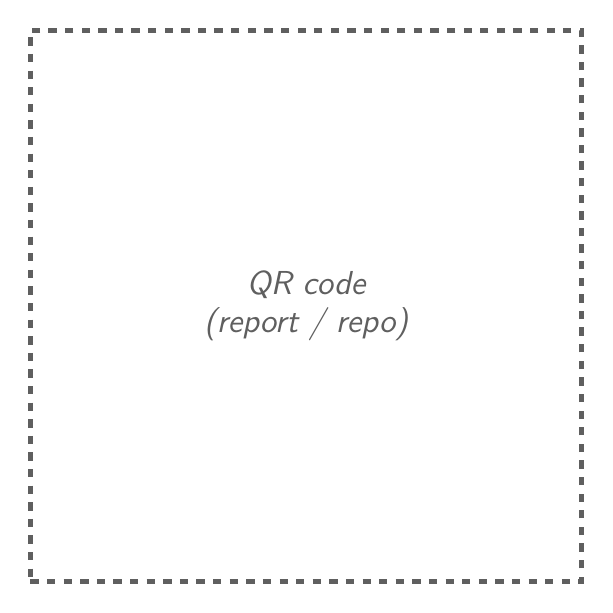
\begin{tikzpicture}
      \node[draw=guidegrey, dashed, line width=2pt, minimum width=7cm,
            minimum height=7cm, text=guidegrey, align=center,
            font=\large\itshape] {QR code\\(report / repo)};
    \end{tikzpicture}%
  }
  \end{center}
  {\small Contact: [email]\\Acknowledgements: [instructor, TAs, resources]}
}
\end{subcolumns}

\end{columns}
\end{document}
